\chapter{Lecture 10: New Revolutions in Particle Physics}

These notes follow Leonard Susskind's tenth lecture in the supplementary Particle Physics 2 sequence, curated by LazyingArt LLC, and keep the lecture's order very close to the board and transcript. The lecture begins by looking forward to the larger puzzles of particle physics, but it quickly turns back to the Higgs for a precise reason: the Higgs is not merely one more particle to be found, but the mechanism that organizes fermion masses, weak-boson masses, and a large part of the phenomenology that the theory predicts. From there the argument moves in a deliberate sequence: first the Dirac Lagrangian, then chirality, then the obstruction to a bare fermion mass in a chiral weak theory, then the Higgs repair of that obstruction, and finally the deeper question of why the symmetry-breaking scale itself is so small.

\section{From Higgs Motivation Back to the Dirac Lagrangian}

Susskind begins by reminding us that the Higgs boson matters because Higgs physics is really the physics of masses and couplings. To make that concrete, he backs up from the Higgs itself and returns to the Dirac equation. Instead of starting from the covariant form immediately, he first writes the older \(\alpha,\beta\) notation on the board. That choice is pedagogically useful: it lets us see the mass term before we tidy the expression into modern form.

\begin{figure}[h]
\centering

\includegraphics[width=0.82\textwidth]{lecture_10_figure_02.png}
\caption{Dirac Lagrangian in \(\alpha,\beta\) notation.}
\end{figure}

In the lecture the chalkboard notation is partly cropped and convention-loose, so we standardize the displayed formula while keeping the stage of the argument intact:
\begin{equation}
\left(\partial_t + \alpha_i \partial_i - \beta m\right)\psi = 0,
\end{equation}
and therefore, by multiplying by \(\psi^\dagger\),
\begin{equation}
\mathcal{L}_D^{(\alpha,\beta)}
=
\psi^\dagger\left(\partial_t + \alpha_i \partial_i - \beta m\right)\psi .
\end{equation}

The lecture's interpretation is as important as the formula. The derivative terms are kinetic terms: they absorb a fermion at one spacetime point and move it to a neighboring point, while also acting on spin. The mass term contains no derivative at all. It absorbs and re-emits the particle at the same point. At this stage one might still think of that as a familiar mass insertion. The point of the lecture is that in a chiral gauge theory it will not remain so innocent.

Susskind then cleans up the notation. Define
\begin{equation}
\bar{\psi}=\psi^\dagger\beta=\psi^\dagger\gamma^0,
\qquad
\gamma^0\equiv \beta,
\qquad
\gamma^i\equiv \beta\alpha_i.
\end{equation}
With these definitions the Dirac Lagrangian takes the schematic covariant form
\begin{equation}
\mathcal{L}_D
=
\bar{\psi}\left(\gamma^0\partial_t+\gamma^i\partial_i+m\right)\psi .
\end{equation}
The board and transcript are a little loose about the visible \(i\) and about sign conventions, so in the notes we standardize once and for all to the canonical modern expression
\begin{equation}
\mathcal{L}_D
=
\bar{\psi}\left(i\gamma^\mu\partial_\mu-m\right)\psi .
\end{equation}

\begin{figure}[h]
\centering

\includegraphics[width=0.82\textwidth]{lecture_10_figure_03.png}
\caption{Covariant gamma-matrix form of the Dirac Lagrangian.}
\end{figure}

This rewrite matters because now the transformation properties are easier to see. In particular, \(\bar{\psi}\psi\) is a scalar, while \(\bar{\psi}\gamma^\mu\psi\) is a four-vector. We are now in position to ask what the mass term actually does.

\section{Chirality and the Meaning of a Dirac Mass}

The next step in the lecture is to introduce the fifth Dirac matrix \(\gamma_5\). Susskind uses it as the chirality operator. It satisfies
\begin{equation}
\gamma_5^2=1,
\end{equation}
so its eigenvalues are \(\pm1\). These two eigenspaces define the left-handed and right-handed parts of the spinor:
\begin{equation}
\psi=\psi_L+\psi_R.
\end{equation}

The key structural point is this: the kinetic part of the Dirac Lagrangian does not mix \(\psi_L\) and \(\psi_R\), but the scalar mass term does. On the board this is exactly the point being emphasized.

\begin{figure}[h]
\centering

\includegraphics[width=0.80\textwidth]{lecture_10_figure_04.png}
\caption{Left-right decomposition of the Dirac mass term.}
\end{figure}

The crucial decomposition is
\begin{equation}
\bar{\psi}\psi
=
\psi_L^\dagger\psi_R+\psi_R^\dagger\psi_L .
\end{equation}
So the Dirac mass term
\begin{equation}
-m\bar{\psi}\psi
=
-m\left(\psi_L^\dagger\psi_R+\psi_R^\dagger\psi_L\right)
\end{equation}
literally flips chirality. It turns a left-handed fermion into a right-handed one and vice versa. In this language a massless fermion has a definite chirality, whereas a massive fermion is constantly being mixed between the two sectors by the mass term.

This is the lecture's first real conceptual tightening. Up to this point the mass term looked familiar. Once we rewrite it in chiral language, it becomes a very specific operator: a left-right mixing operator. That is precisely what will run into trouble when weak interactions are recalled to be chiral.

\section{Weak Interactions and the Forbidden Mass Term}

Now the lecture pivots. The weak interaction, more precisely the \(W\)-boson interaction, couples only to left-handed fermions. Susskind briefly says \(Z\) and then corrects himself; the corrected physics is the important one. With respect to the weak \(SU(2)\) symmetry under discussion, the left-handed fermion transforms nontrivially, while the right-handed fermion is uncharged.

But the Dirac mass term takes a left-handed charged object into a right-handed uncharged one. In a gauge theory that is not a harmless change of notation; it is a violation of the transformation law that the Lagrangian must respect. The problem is not that the algebra failed. The problem is that the naive mass term is not gauge-legal in the chiral weak theory.

\subsection{Question \& Answer}

\paragraph{Question.} How can fermions be massive if the weak interaction couples only to left-handed fields?

\paragraph{Answer.} A bare Dirac mass term cannot do the job, because it directly couples \(\psi_L\) to \(\psi_R\), and those two fields do not carry the same weak quantum numbers. What we need is an additional field that carries the mismatch in weak charge. The Higgs field provides exactly that missing ingredient.

This is one of the lecture's characteristic moves. A familiar textbook term is not merely written down; it is turned into a puzzle by the symmetry structure of the Standard Model. Only after that obstruction is made sharp does the Higgs enter.

\section{Higgs Insertion, Yukawa Couplings, and Observable Consequences}

The Higgs field enters as the charged object that can make the left-right coupling legitimate. Susskind keeps the discussion schematic. He notes that the Higgs is itself a weak doublet, but he does not pause to develop the full component structure. The important board-level statement is simply that the Higgs field \(\phi\) must be inserted between the left-handed and right-handed fermions:
\begin{equation}
\mathcal{L}_Y
=
G_Y\left(\psi_L^\dagger \phi\,\psi_R+\psi_R^\dagger \phi^\dagger \psi_L\right).
\end{equation}
Here \(G_Y\) is the Yukawa coupling, a dimensionless number, and in general each fermion species has its own such number.

Now comes the second decisive move. Because of spontaneous symmetry breaking, the Higgs field does not sit at the origin. Instead we write
\begin{equation}
\phi = F + H,
\end{equation}
where \(F\) is the nonfluctuating part, the shifted vacuum value, and \(H\) is the fluctuating Higgs field itself. Substituting this into the Yukawa term gives
\begin{align}
\mathcal{L}_Y
&=
G_Y\left(\psi_L^\dagger (F+H)\psi_R+\psi_R^\dagger (F+H)^\dagger \psi_L\right) \\
&=
G_YF\left(\psi_L^\dagger\psi_R+\psi_R^\dagger\psi_L\right)
+
G_YH\left(\psi_L^\dagger\psi_R+\psi_R^\dagger\psi_L\right).
\end{align}
The first piece is a fermion mass term, so
\begin{equation}
m_f = G_Y F.
\end{equation}
The second piece is a genuine Higgs-fermion interaction.

This is the essential repair. The forbidden bare mass term is replaced by a gauge-invariant Yukawa interaction, and once the Higgs field acquires its vacuum value, the mass term reappears effectively. But it is no longer put in by hand as an isolated term; it is generated by the symmetry-breaking background.

The lecture then leans immediately into phenomenology. The same \(F\) that determines the \(W\) and \(Z\) masses also enters the fermion masses. Once the weak-boson masses are known, \(F\) is known to be of order a few hundred \(\mathrm{GeV}\), roughly
\begin{equation}
F \sim 200\,\mathrm{GeV}.
\end{equation}
Then the observed fermion masses tell us the Yukawa couplings. A light electron means a tiny Yukawa coupling; a heavy top quark means a large one.

And because the Higgs interaction is proportional to the same \(G_Y\), the decay pattern of the Higgs is not arbitrary. The couplings that generate masses are the couplings that control Higgs emission and Higgs decay. That is why Susskind insists that discovering the Higgs is more than discovering one particle. It is the discovery of a whole structure of interactions.

\section{The Mexican-Hat Potential and the Scale \(F\)}

Having explained how the Higgs generates masses, the lecture immediately asks the next question: what determines the Higgs field itself? Here the dynamics is encoded in the potential.

\begin{figure}[h]
\centering

\includegraphics[width=0.82\textwidth]{lecture_10_figure_05.png}
\caption{Higgs-inserted chiral coupling and double-well potential.}
\end{figure}

Near the origin the potential must be an upside-down parabola, so Susskind writes it in the form
\begin{equation}
V(\phi)
=
-\frac{\mu^2}{2}\phi^2+\frac{\lambda}{4}\phi^4.
\end{equation}
The meaning of the terms is clear from the lecture's pacing. The negative quadratic term destabilizes the origin. If that were all we had, the field would run off to infinity and there would be no ground state. The quartic term is the simplest even term that restores stability at large \(|\phi|\). Odd powers would spoil the symmetry between \(+\phi\) and \(-\phi\), so the quartic is the natural next step.

\begin{figure}[h]
\centering
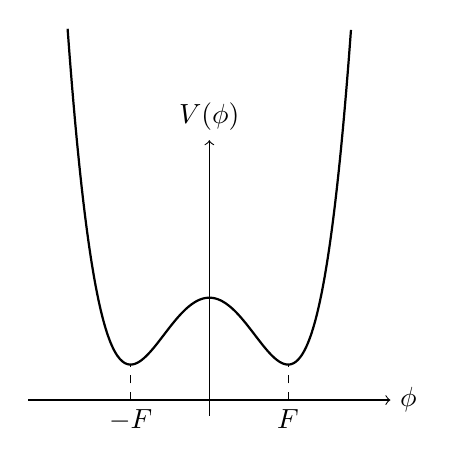
\begin{tikzpicture}[scale=1.0]
\draw[->] (-2.3,0) -- (2.3,0) node[right] {\(\phi\)};
\draw[->] (0,-0.2) -- (0,3.3) node[above] {\(V(\phi)\)};
\draw[thick, smooth, domain=-1.8:1.8, samples=120] plot (\x,{0.85*(\x*\x-1)^2 + 0.45});
\draw[dashed] (-1,0) -- (-1,0.45);
\draw[dashed] (1,0) -- (1,0.45);
\node[below] at (-1,0) {\(-F\)};
\node[below] at (1,0) {\(F\)};
\end{tikzpicture}
\caption{A one-dimensional cross-section through the symmetry-breaking potential.}
\end{figure}

Now we can carry out the minimization explicitly. This is one of the places where the lecture really does a worked calculation rather than only gesturing:
\begin{align}
\frac{dV}{d\phi}
&=
-\mu^2\phi+\lambda\phi^3 = 0, \\
\phi\left(-\mu^2+\lambda\phi^2\right) &= 0.
\end{align}
So away from the unstable solution \(\phi=0\), the minima satisfy
\begin{equation}
\phi^2=\frac{\mu^2}{\lambda}.
\end{equation}
The shifted vacuum value is therefore
\begin{equation}
F^2=\frac{\mu^2}{\lambda}.
\end{equation}

The lecture's qualitative emphasis should be preserved here. \(\lambda\) is treated as an ordinary dimensionless coupling, not as an absurdly tiny number. The scale is really being set by \(\mu\), and therefore by \(F\). Both \(\mu\) and \(F\) have dimensions of mass. Once that scale is chosen, many of the particle masses we observe are dragged along with it.

\section{Why Are the Observed Masses All Tied to \(F\)?}

At this point the lecture broadens again. Why should so many known particles have masses proportional to one and the same symmetry-breaking scale? The answer is partly structural. Particles whose left-handed and right-handed components transform differently under the weak interaction cannot have a bare mass. Their masses must vanish if the Higgs field has no shift, and therefore when they do acquire mass it must be proportional to \(F\).

But that need not be true of every possible particle. One could imagine particles whose left-handed and right-handed components transform in the same way under the weak symmetry. One could also imagine particles with no weak interaction at all. Such particles could have perfectly respectable mass terms that do not involve \(\phi\), and their masses would then have no reason to track the electroweak scale.

That point is essential to the hierarchy problem as Susskind frames it. The observed light spectrum may be light precisely because these are the particles whose masses are forced to depend on \(F\). Other particles, not so constrained, might naturally sit at very high mass scales and would therefore be hard to detect. The strange number in the room is not the large scale. The strange number is the small one.

Before the break Susskind gives a condensed-matter analogy that should be kept, but kept in its proper place. In superfluidity or Bose condensation a field acquires a shifted value. In a superconductor the relevant condensed object is charged, and the analogy becomes closer to the Higgs mechanism itself: the photon effectively acquires a finite penetration depth, and the whole phenomenon looks very much like a laboratory version of spontaneous gauge-symmetry breaking. This is illuminating, but it is not a replacement for the mathematical argument above. It is an intuition for the same pattern.

So the local problem has been solved. We know how fermion masses arise. We know how the Higgs field enters. We know how the shift \(F\) is extracted. The next question is larger: small compared with what? What is the natural scale against which \(F\) is to be judged?

\section{Renormalization, Running Couplings, Unification, and the Return of the Hierarchy Puzzle}

After the break the lecture changes altitude. We now think not only about particle content, but about parameters. The parameters written into the Lagrangian are inputs, but the experimentally measured masses and couplings are dressed by the interactions of the vacuum. The simplest illustration is electric charge.

\paragraph{QED screening.}
At large distance the Coulomb law defines the observed electric charge:
\begin{equation}
V_{\mathrm{Coulomb}}(r)\sim \frac{e^2(r)}{r},
\qquad
F_{\mathrm{Coulomb}}(r)\sim \frac{e^2(r)}{r^2}.
\end{equation}
In matter this is familiar from conductors and dielectrics: surrounding charges polarize and partially screen the source. In quantum electrodynamics the vacuum itself plays the role of a dielectric. Virtual electron-positron pairs are polarized by the electric field, so the charge measured at large distances is smaller than the short-distance charge. As one probes smaller \(r\), more of the screening cloud is peeled away. Thus \(e(r)\) grows as \(r\) decreases, or equivalently as \(1/r\) increases. The lecture emphasizes that this growth is only logarithmic, but it is real.

\paragraph{QCD antiscreening.}
For the strong interaction the story reverses. Gluons interact with gluons, and the chromoelectric flux lines attract one another. At large distance the flux is squeezed into a tube and the potential becomes approximately linear:
\begin{equation}
V_{\mathrm{QCD}}(r)\propto r.
\end{equation}
Equivalently, the effective strong coupling becomes larger at large separation and smaller at short distance. So if we plot couplings against inverse distance, the QED coupling creeps upward, while the QCD coupling falls.

\paragraph{Weak coupling and unification.}
The weak coupling runs in between these two behaviors. Susskind's point is qualitative but powerful: if one takes the measured couplings at accessible energies and runs them upward using the Standard Model, the strong, weak, and electromagnetic couplings come close to meeting. In supersymmetric extensions they come together more sharply, at an energy scale of order
\begin{equation}
\mu_{\mathrm{unif}}\sim 10^{16}\,\mathrm{GeV}.
\end{equation}
That is not yet a proof of unification, but it is exactly the kind of numerical conspiracy that suggests a deeper structure.

\begin{figure}[h]
\centering
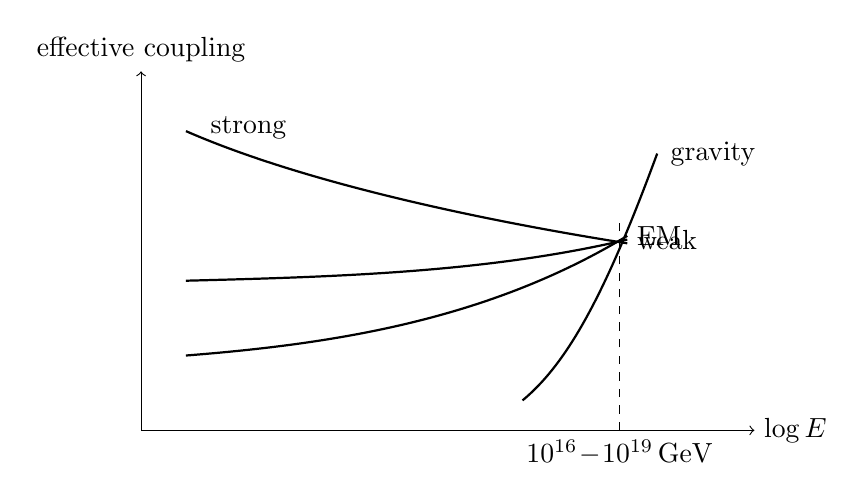
\begin{tikzpicture}[scale=0.95]
\draw[->] (0,0) -- (8.2,0) node[right] {\(\log E\)};
\draw[->] (0,0) -- (0,4.8) node[above] {effective coupling};

\draw[thick] (0.6,1.0) .. controls (2.5,1.15) and (4.6,1.45) .. (6.5,2.6);
\node[right] at (6.5,2.6) {EM};

\draw[thick] (0.6,2.0) .. controls (2.5,2.05) and (4.6,2.1) .. (6.5,2.55);
\node[right] at (6.5,2.55) {weak};

\draw[thick] (0.6,4.0) .. controls (2.2,3.3) and (4.6,2.8) .. (6.5,2.5);
\node[right] at (0.8,4.05) {strong};

\draw[thick] (5.1,0.4) .. controls (5.7,0.9) and (6.2,1.8) .. (6.9,3.7);
\node[right] at (6.95,3.7) {gravity};

\draw[dashed] (6.4,0) -- (6.4,2.8);
\node[below] at (6.4,0) {\(10^{16}\!-\!10^{19}\,\mathrm{GeV}\)};
\end{tikzpicture}
\caption{Qualitative running of the gauge couplings, together with the heuristic rise of gravity at short distance.}
\end{figure}

\paragraph{Short-distance gravity.}
The lecture then adds gravity in a heuristic way. Ordinarily Newton's force law is
\begin{equation}
F_G \sim \frac{Gm_1m_2}{r^2}.
\end{equation}
But for relativistic particles the relevant source is energy, not merely rest mass, so one replaces \(m\) by \(E/c^2\):
\begin{equation}
F_G(r)\sim \frac{GE^2}{c^4r^2}.
\end{equation}
Now use the uncertainty-principle estimate for particles localized within distance \(r\):
\begin{equation}
p\sim \frac{\hbar}{r},
\qquad
E\sim pc\sim \frac{\hbar c}{r}.
\end{equation}
Substituting this into the gravitational force estimate gives
\begin{equation}
F_G(r)\sim \frac{G}{c^4r^2}\left(\frac{\hbar c}{r}\right)^2
\sim
\frac{G\hbar^2}{c^2r^4}.
\end{equation}
So at very short distances gravity grows more rapidly than the ordinary Coulomb force. If we compare this with \(F_{\mathrm{Coulomb}}(r)\sim e^2/r^2\), the crossover occurs at the characteristic length
\begin{equation}
r_P \sim \sqrt{\frac{G\hbar}{c^3}},
\end{equation}
up to the dimensionless electromagnetic coupling and the rough numerical simplifications Susskind makes on the board. This is the Planck length.

Now the lecture closes the circle. Once one admits very high scales such as the unification scale or the Planck scale, the real mystery is no longer why those scales are large. Those are the scales that begin to look natural. The mystery is why the electroweak scale, encoded in \(F\), is so small by comparison. Why is the one number that controls the masses of the \(W\), the \(Z\), the quarks, and the charged leptons so much smaller than the ultraviolet scales that the running couplings seem to be pointing toward? That is the hierarchy problem in the lecture's sense. It is left deliberately unresolved, but much more sharply posed than it was at the beginning.

\section{Summary}

The lecture's mathematical line is clear once we preserve its order. We start from the Dirac Lagrangian, recognize that the mass term mixes chirality, and then discover that such a term is forbidden in the chiral weak theory unless a Higgs field is inserted to carry the weak charge. After the Higgs field shifts by \(F\), the Yukawa interaction produces fermion masses \(m_f=G_YF\) and at the same time predicts Higgs couplings and decay patterns. The Higgs potential determines \(F\) through \(F^2=\mu^2/\lambda\), but that local success opens the larger question: why should \(F\) be so small at all? The second half of the lecture then supplies the ultraviolet setting for that question by introducing running couplings, approximate unification, and the Planck scale. In that broader setting the puzzle is sharpened rather than solved: if very high mass scales are natural, the small electroweak scale is what demands explanation.